\documentclass[xcolor=dvipsnames]{beamer}
\usetheme{Madrid}
\useoutertheme{infolines}
\useinnertheme{circles}
\setbeamertemplate{navigation symbols}{}
\usepackage[utf8]{inputenc}
\usepackage[absolute,overlay]{textpos}
\usepackage{amsmath,array}
\usepackage{amsthm}
\usepackage{amssymb}
\usepackage{bm}
\setbeamertemplate{caption}[numbered]
\usepackage{caption}
\usepackage{color}
\usepackage[force]{feynmp-auto} %<-added force
\usepackage{float}
\usepackage{graphicx}
\usepackage{hyperref}
\usepackage{lipsum}
\usepackage{listings}
\usepackage{mathtools}
\usepackage{mdframed}
\usepackage[version=4]{mhchem}
\usepackage{physics}
\usepackage{setspace}
\usepackage{subcaption}
\usepackage{tikz}
\usetikzlibrary{decorations.pathreplacing} % For curly braces
\usepackage{xcolor}

% Set colours
\definecolor{bgblue}{rgb}{0.05, 0.15, 0.3}
\setbeamercolor{palette primary}{bg=bgblue,fg=white}
\setbeamercolor{palette secondary}{bg=bgblue,fg=white}
\setbeamercolor{palette tertiary}{bg=bgblue,fg=white}
\setbeamercolor{palette quaternary}{bg=bgblue,fg=white}
\setbeamercolor{structure}{fg=bgblue}
\setbeamercolor{section in toc}{fg=bgblue}

\hypersetup{
    colorlinks=true, % coloured links instead of boxes
    linkcolor=orange, % colour of internal links
    citecolor=blue, % colour of citation links
    urlcolor=blue % colour of URLs
}

\definecolor{codegreen}{rgb}{0,0.6,0}
\definecolor{codegray}{rgb}{0.5,0.5,0.5}
\definecolor{codepurple}{rgb}{0.6,0,0.8}
\definecolor{backcolour}{rgb}{0.95,0.95,0.9}
\lstdefinestyle{mystyle}{
    backgroundcolor=\color{backcolour}, commentstyle=\color{codegreen},
    keywordstyle=\color{magenta},
    numberstyle=\tiny\color{codegray},
    stringstyle=\color{codepurple},
    basicstyle=\ttfamily\footnotesize,
    breakatwhitespace=false,         
    breaklines=true,                 
    captionpos=b,                    
    keepspaces=true,                 
    numbers=left,                    
    numbersep=5pt,                  
    showspaces=false,                
    showstringspaces=false,
    showtabs=false,                  
    tabsize=2
}
\lstset{style=mystyle}
\renewcommand{\lstlistingname}{Program}

\renewcommand{\qed}{\hspace{1.2ex}\blacksquare}
\renewcommand{\cite}[1]{\textbf{[\onlinecite{#1}]}}
\def\R{\mathbb{R}}
\def\Q{\mathbb{Q}}
\def\N{\mathbb{N}}
\def\C{\mathbb{C}}
\def\Z{\mathbb{Z}}
\def\a{\alpha}
\def\b{\beta}
\def\c{\gamma}
\def\d{\delta}
\def\D{\Delta}
\def\e{\varepsilon}
\def\l{\lambda}
\def\s{\sigma}
\def\t{\tau}
\def\w{\omega}
\def\W{\Omega}
\def\La{\mathcal{L}}
\def\Ld{\Lambda}
\def\M{\mathcal{M}}
\def\bigO{\mathcal{O}}
\def\p{\partial}
\def\n{\nabla}
\def\iff{\Longleftrightarrow}
\def\rank{\text{rank}}
\def\Tr{\text{Tr}}
\renewcommand\abstractname{\textbf{Abstract}}
\def\andname{\hspace{-0.2em},}
\allowdisplaybreaks

\newcommand{\br}[1]{
  \begin{textblock*}{\textwidth}(0pt,\textheight-15pt)
    \raggedleft
    \small{(#1)}
  \end{textblock*}
}

\title[Observation of Charge-Parity Symmetry Breaking in Baryon Decays]{\textbf{Observation of Charge-Parity Symmetry Breaking in Baryon Decays (LHCb collaboration, 2025)}}
\date{April 24, 2025}
\author[Mingrui ZHOU, Kelvin YUE]{Mingrui ZHOU, Kelvin YUE}
\institute[]{Department of Physics, HKUST}

\begin{document}
\frame{\titlepage}

% Overview frame with custom ToC
\begin{frame}{Overview}
    \tableofcontents
      \begin{tikzpicture}[overlay, remember picture]
        \draw[black, thick, decorate, decoration={brace, amplitude=10pt}]
          ([xshift=1.5cm, yshift=2.7cm]current page.center) -- 
          ([xshift=1.5cm, yshift=0.7cm]current page.center);
        \node[text=black, right, align=center, text width=3cm] at ([xshift=1cm, yshift=1.7cm]current page.center) {Mingrui};
      \end{tikzpicture}
      A review of \url{https://arxiv.org/abs/2503.16954} (LHCb collaboration, 2025).
\end{frame}

% Define sections
\section{CP Violation in SM Flavour Physics}
\section{Direct and Indirect Detection Methodology}
\section{Milestones in CP Violation Detection}

\section{Theoretical Framework for Baryon Decay}
\begin{frame}{4. Theoretical Framework for Baryon Decay}
\textbf{Process}\\
\begin{itemize}
    \item Compare $\Ld_{b}^{0}\to p K^{-}\pi^{-}\pi^{+}$ and its conjugate $\bar{\Ld}_{b}^{0}\to \bar{p}K^{+}\pi^{+}\pi^{-}$
\end{itemize}
\begin{minipage}[t]{0.45\textwidth}
\begin{figure}
    \centering
    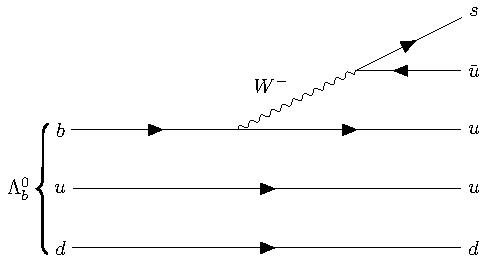
\includegraphics[width=\linewidth]{lambdab_tree.pdf}
\end{figure}
\end{minipage}
\begin{minipage}[t]{0.45\textwidth}
\begin{figure}
    \centering
    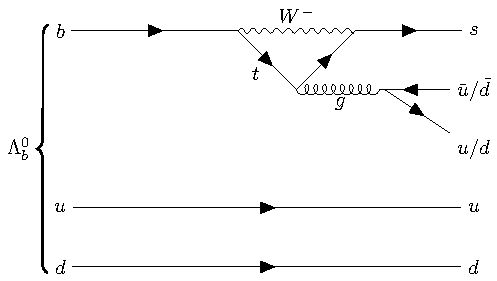
\includegraphics[width=\linewidth]{lambdab_loop.pdf}
\end{figure}
\end{minipage}
\begin{itemize}
    \item Amount of CP violation is quantified by relative difference between decay rates:
    \begin{align*}
        \mathcal{A}_{CP}\equiv\frac{\Gamma(\Ld_{b}^{0}\to p K^{-}\pi^{-}\pi^{+})-\Gamma(\bar{\Ld}_{b}^{0}\to \bar{p}K^{+}\pi^{+}\pi^{-})}{\Gamma(\Ld_{b}^{0}\to p K^{-}\pi^{-}\pi^{+})+\Gamma(\bar{\Ld}_{b}^{0}\to \bar{p}K^{+}\pi^{+}\pi^{-})}
    \end{align*}
\end{itemize}
\end{frame}

\begin{frame}{4. Theoretical Framework for Baryon Decay}
\textbf{Tree-level Process}
\begin{itemize}
    \item $b\to u W^{-}$: vertex $\propto$ $V_{ub}\approx A\l^{3}(\rho-i\eta)$
    \item $W^{-}\to \bar{u}s$: vertex $\propto$ $V_{us}^\ast\approx \l^\ast$
    \item Total CKM factor: $\propto$ $V_{ub}V_{us}^\ast$, weak phase $\phi_{T}=\arg(V_{ub}V_{us}^\ast)\approx -65.4^\circ$
\end{itemize}
\begin{figure}
    \centering
    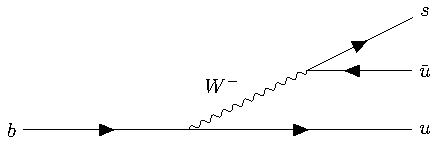
\includegraphics[width=0.6\linewidth]{b_tree.pdf}
\end{figure}
\end{frame}

\begin{frame}{4. Theoretical Framework for Baryon Decay}
\textbf{Loop-level Process}\\
\begin{itemize}
    \item Flavour-changing neutral current (FCNC) process
    \item Suppressed at tree-level in the SM, since $Z$ boson and gluon do not change flavour
    \item $b\to s$ transition via a loop with a $W^{-}$ boson and internal quark $t$
    \item Emission of a gluon from the loop, which produces the $u\bar{u}$ pair
\end{itemize}
\begin{figure}
    \centering
    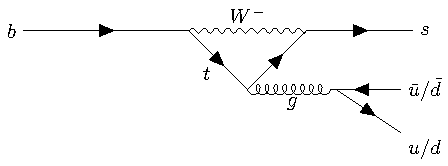
\includegraphics[width=0.6\linewidth]{b_loop.pdf}
\end{figure}
\end{frame}

\begin{frame}{4. Theoretical Framework for Baryon Decay}
\textbf{Loop-level Process (cont.)}\\
\begin{itemize}
    \item $b\to tW^{-}$: vertex $\propto$ $V_{tb}\approx -A\l^2$
    \item $tW^{-}\to s$: vertex $\propto$ $V_{ts}^\ast\approx 1$
    \item Total CKM factor: $\propto$ $V_{tb}V_{us}^\ast$, weak phase $\phi_{L}=\arg(V_{tb}V_{us}^\ast)\approx 0$
\end{itemize}
\begin{figure}
    \centering
    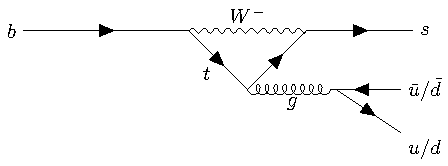
\includegraphics[width=0.6\linewidth]{b_loop.pdf}
\end{figure}
\end{frame}

\begin{frame}{4. Theoretical Framework for Baryon Decay}
\textbf{Interference between Tree and Loop Amplitudes}\\
\begin{itemize}
    \item Amplitude of decays:
    \begin{align*}
        A(\Ld_{b}^{0})&=|A_{T}|e^{+i\phi_{T}}e^{i\d_{T}}+|A_{L}|e^{+i\phi_{L}e^{i\d_{L}}}\\
        A(\bar{\Ld}_{b}^{0})&=|A_{T}|e^{\textcolor{red}{-}i\phi_{T}}e^{i\d_{T}}+|A_{L}|e^{\textcolor{red}{-}i\phi_{L}e^{i\d_{L}}}
    \end{align*}
    \item Weak phases $\phi_{T/L}$: defined by CKM elements $V_{ub}V_{us}^\ast$ and $V_{tb}V_{ts}^\ast$
    \item Strong phases $\d_{T/L}$: process-dependent, difficult to calculate due to non-perturbative QCD effects at low energies
\end{itemize}
\br{M. Beneke+, 1999}
\end{frame}

\begin{frame}{4. Theoretical Framework for Baryon Decay}
\textbf{Interference between Tree and Loop Amplitudes (cont.)}\\
\begin{itemize}
    \item Decay rate $\Gamma\propto |A|^{2}$, so
    \begin{align*}
        \mathcal{A}_{CP}=\frac{|A(\Ld_{b}^{0})|^{2}-|A(\bar{\Ld}_{b}^{0})|^{2}}{|A(\Ld_{b}^{0})|^{2}+|A(\bar{\Ld}_{b}^{0})|^{2}}=\frac{2\sin\D\d\sin\D\phi}{|A_{T}/A_{L}|+|A_{L}/A_{T}|+2\cos\D\d\cos\D\phi},
    \end{align*}
    where $\D\phi=\phi_{T}-\phi_{L}\approx -65.7^\circ$, $\D\d=\d_{T}-\d_{L}$
    \item Sizable $\mathcal{A}_{CP}$ requires $A_{T}\sim A_{L}$, big $\D\phi$ and $\D\d$
\end{itemize}
\end{frame}

\section{Experimental Approach and Results}
\begin{frame}{5. Experimental Approach and Results}
\textbf{Data and Bias}\\
\begin{itemize}
    \item $\Ld_{b}^{0}$ and $\bar{\Ld}_{b}^{0}$ produced in proton-proton ($pp$) collisions
    \item Data collected by the Large Hadron Collider (LHC) from 2011 to 2018, total integrated luminosity $\sim 9\mathrm{fb}^{-1}$
    \item Yield asymmetry: difference of numbers ($N$) of observed decays, defined as
    \begin{align*}
        \mathcal{A}_{N}\equiv\frac{N(\Ld_{b}^{0}\to p K^{-}\pi^{-}\pi^{+})-N(\bar{\Ld}_{b}^{0}\to \bar{p}K^{+}\pi^{+}\pi^{-})}{N(\Ld_{b}^{0}\to p K^{-}\pi^{-}\pi^{+})+N(\bar{\Ld}_{b}^{0}\to \bar{p}K^{+}\pi^{+}\pi^{-})}
    \end{align*}
\end{itemize}
$\mathcal{A}_{N}\neq\mathcal{A}_{CP}$.
\end{frame}

\begin{frame}{5. Experimental Approach and Results}
\textbf{Data and Bias (cont.)}\\
\begin{itemize}
    \item Production asymmetry: $\s(\Ld_{b}^{0})>\s(\bar{\Ld}_{b}^{0})$ in $pp$ collisions. Protons contain more valence quarks ($u, d$) than antiquarks ($\bar{u}$, $\bar{d}$)\\
    $\implies$ $b$ combines with the proton’s valence $u$ and $d$ more readily to form a $\Ld_{b}^{0}$
    \begin{figure}
        \centering
        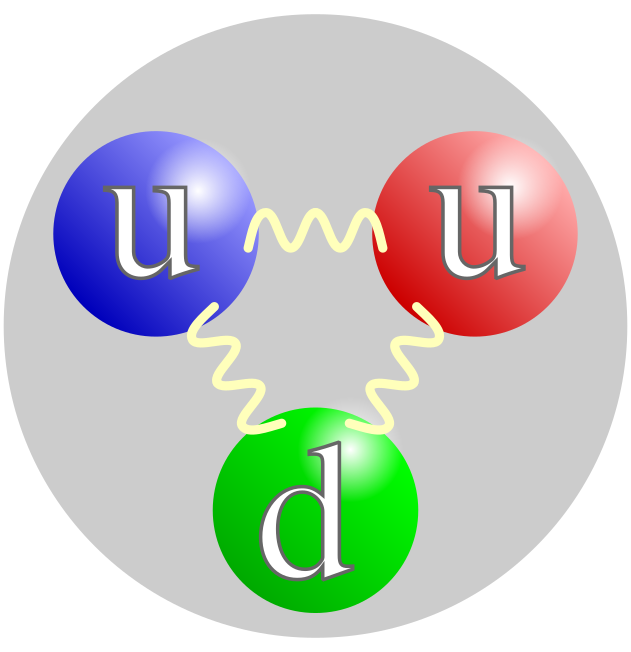
\includegraphics[width=0.2\linewidth]{Quark_structure_proton.png}
    \end{figure}
    \item Detection asymmetry: particles and antiparticles interact with the detector material differently
\end{itemize}
\end{frame}

\begin{frame}{5. Experimental Approach and Results}
\textbf{Control Channel}\\
\begin{itemize}
    \item $\Ld_{b}^{0}\to \Ld_{c}^{+}\pi^{-}$ with $\Ld_{c}^{+}\to p K^{-}\pi^{+}$, dominated by the tree-level $b\to cud$ transition
    \item Its asymmetry reflects only nuisance effects
    \item Subtracted from the signal channel’s yield asymmetry to obtain $\mathcal{A}_{CP}$
\end{itemize}
\begin{figure}
    \centering
    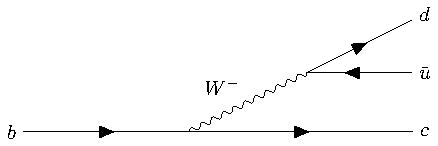
\includegraphics[width=0.5\linewidth]{control_b.pdf}
\end{figure}
\end{frame}

\begin{frame}{5. Experimental Approach and Results}
\textbf{Event Selection}\\
\begin{itemize}
    \item Reduce background from random combinations of final-state particles
    \item Decay vertex is displaced from the $pp$ collision point, since $\Ld_{b}^{0}$ has a long lifetime
    \item High $p_{T}$ for final-state particles due to large $\Ld_{b}^{0}$ mass
    \item Particle identification (PID) reduces misidentification (e.g. $\pi^{-}$ reconstructed as $K^{-}$ in $\Ld_{b}^{0}\to p\pi^{-}\pi^{+}\pi^{-}$)
    \item Mass distributions are fit to extract signal yields, with a peak at $m_{\Ld_{b}^{0}}\approx 5619\mathrm{MeV}/c^{2}$
\end{itemize}
\end{frame}

\begin{frame}{5. Experimental Approach and Results}
\begin{minipage}[t]{0.45\textwidth}
\begin{figure}
    \centering
    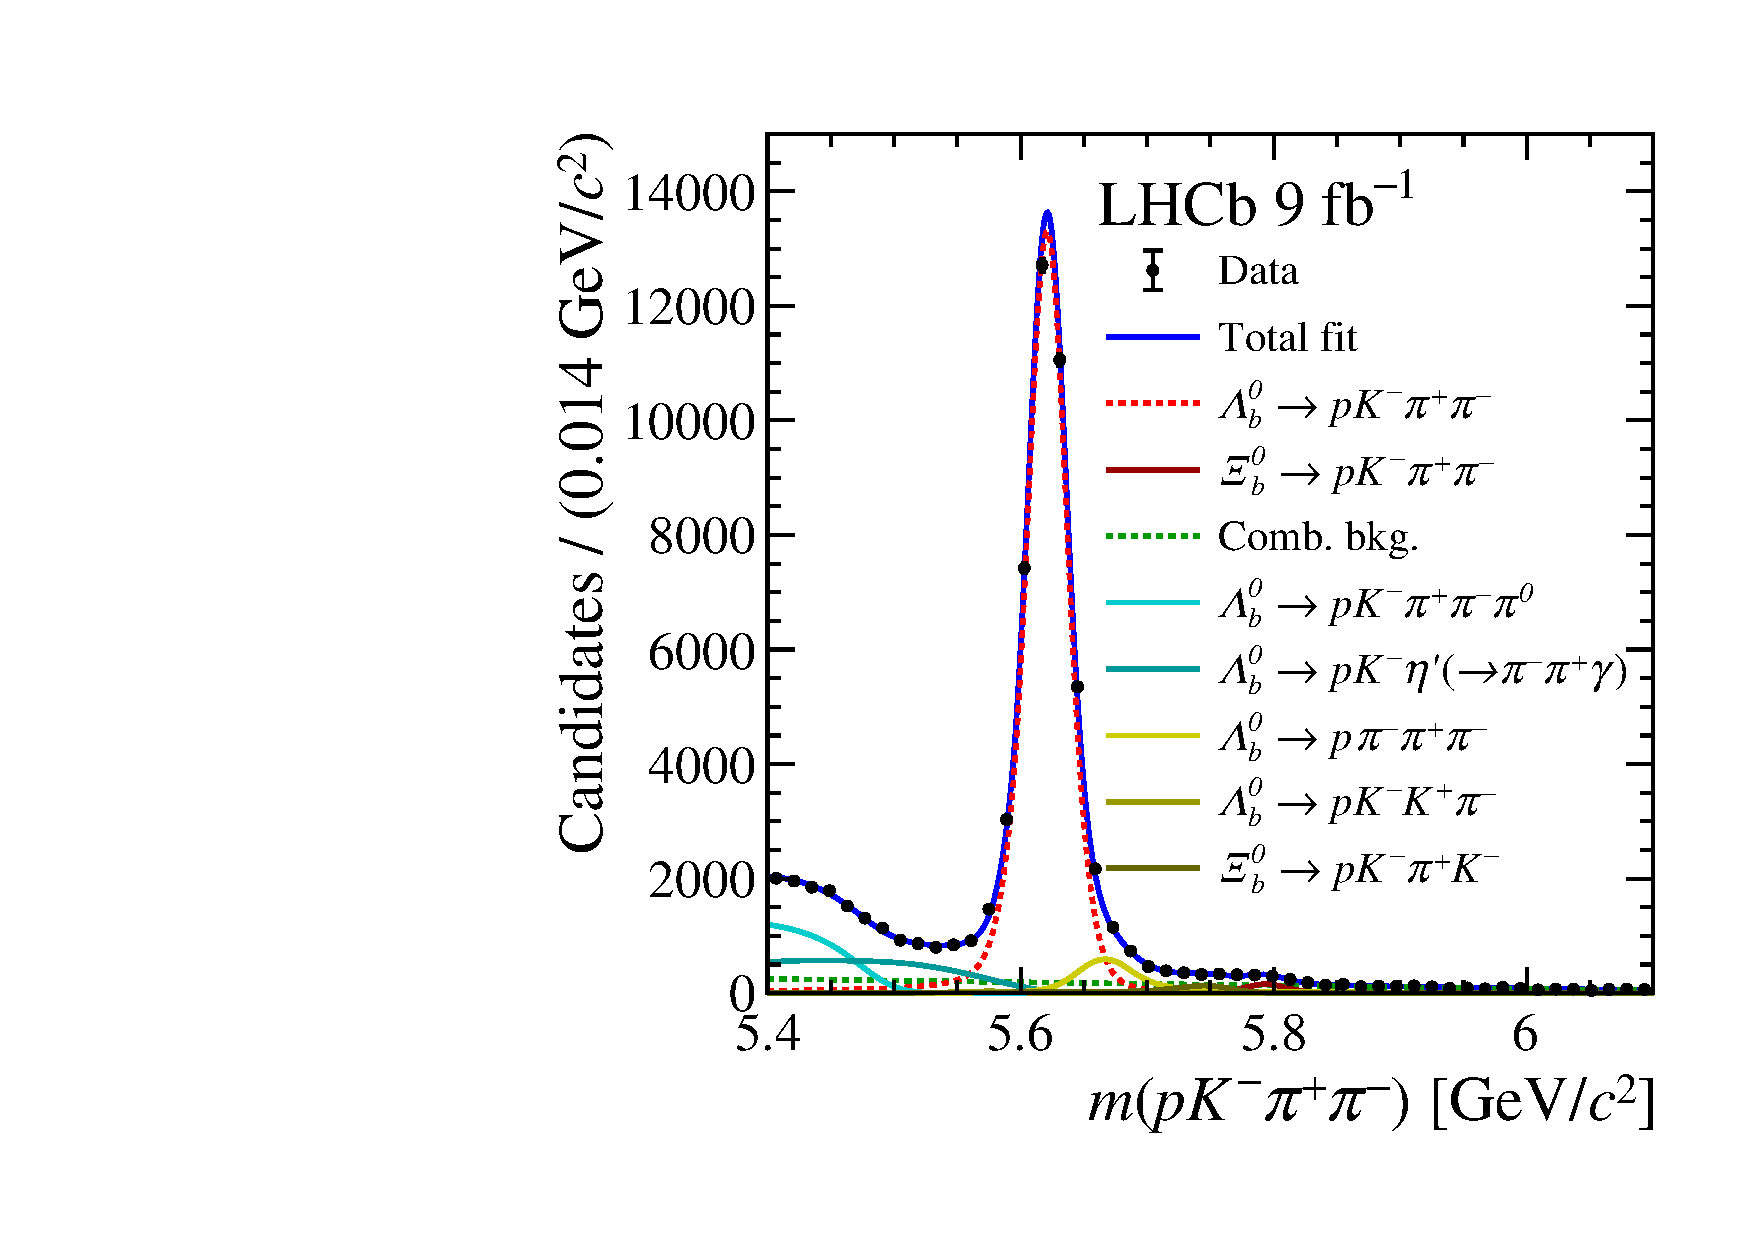
\includegraphics[width=\linewidth]{Fig2a.pdf}
\end{figure}
\end{minipage}
\begin{minipage}[t]{0.45\textwidth}
\begin{figure}
    \centering
    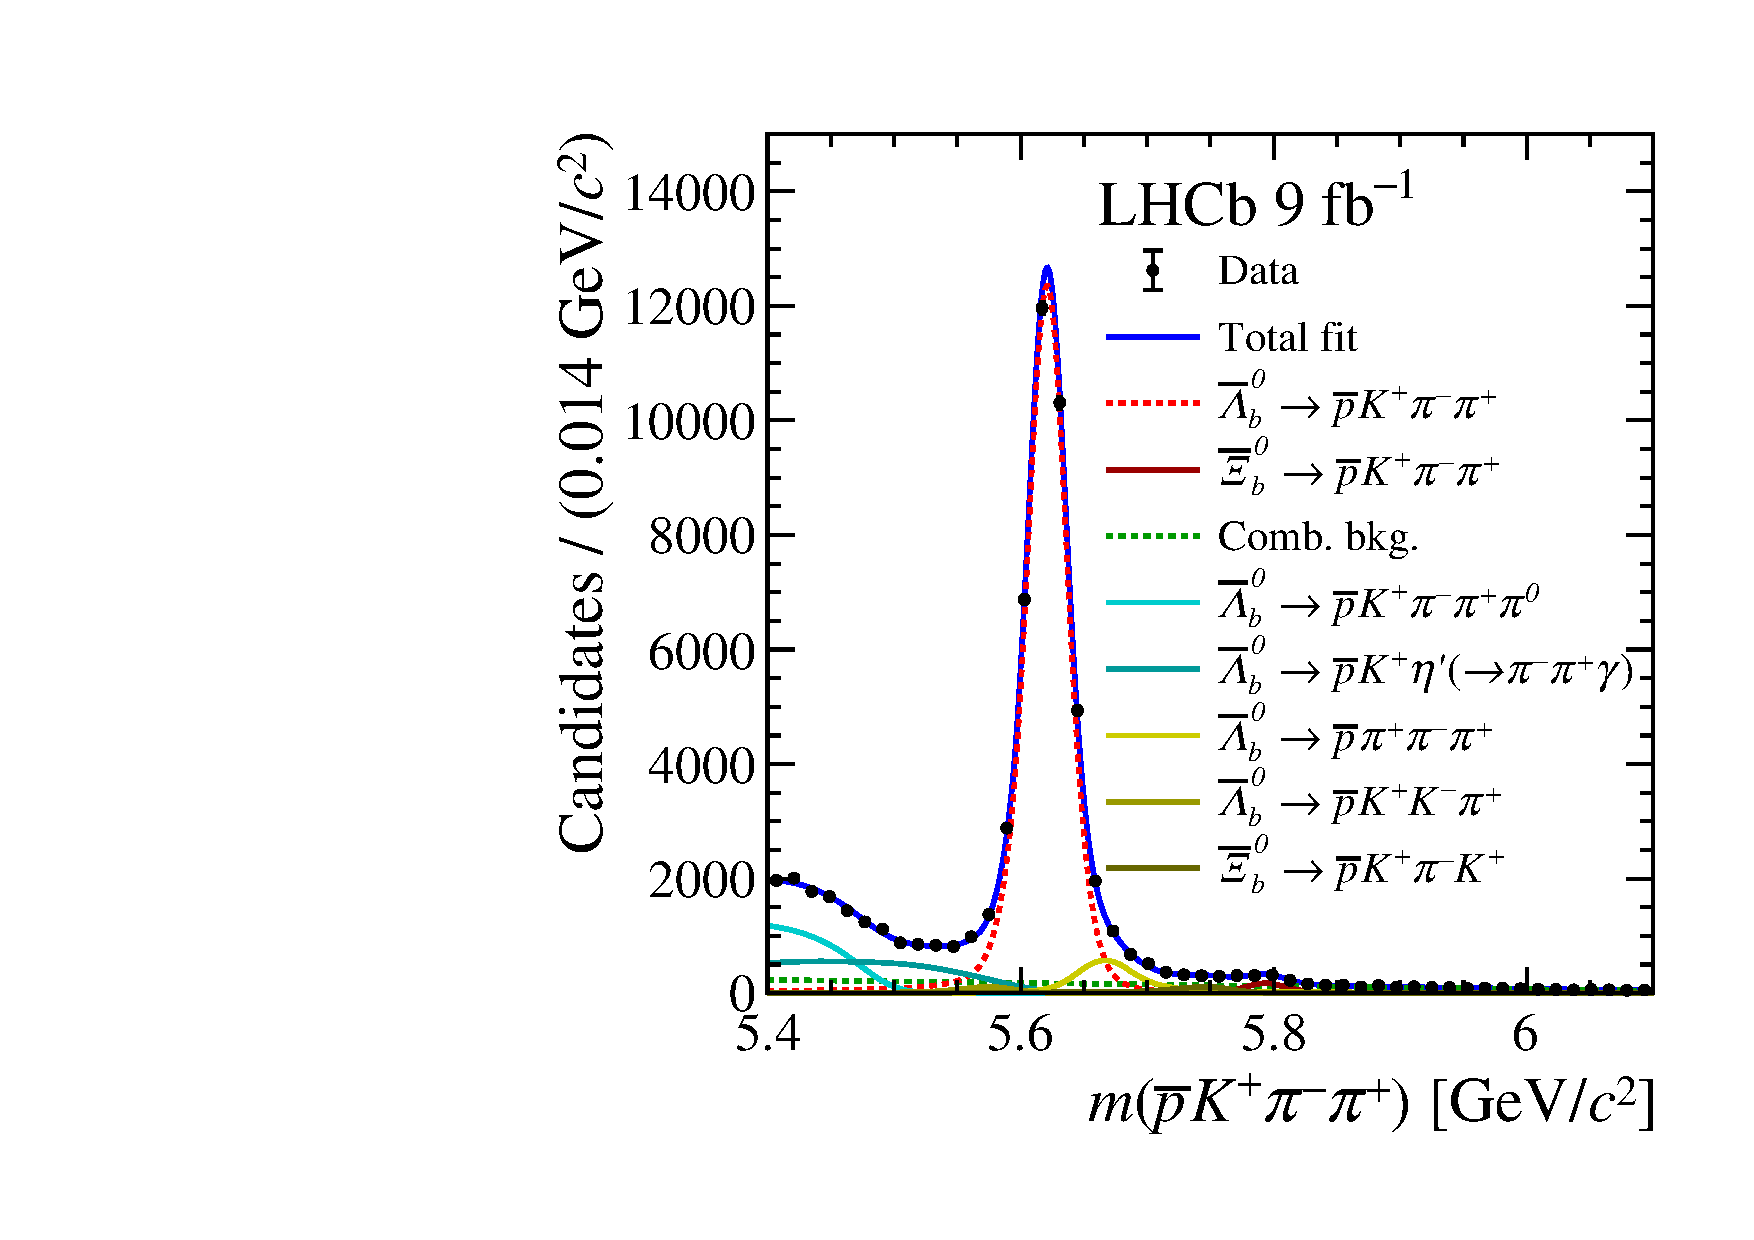
\includegraphics[width=\linewidth]{Fig2b.pdf}
\end{figure}
\end{minipage}
\begin{align*}
    \mathcal{A}_{CP}=(2.45\pm0.46\pm0.10)\% \quad (5.2\s)
\end{align*}
\end{frame}

\begin{frame}{5. Experimental Approach and Results}
\textbf{Phase-Space Analysis}\\
\begin{itemize}
    \item The $\Ld_{b}^{0}\to pK^{-}\pi^{+}\pi^{-}$ decay involves multiple intermediate resonances, identified by two/three-body invariant masses
    \item $\Ld_{b}^{0}\to R(p\pi^{+}\pi^{-})K^{-}$: $\mathcal{A}_{CP}=(5.4\pm 0.9\pm 0.1)\% \quad (6.0\s)$
    \item $\Ld_{b}^{0}\to R(pK^{-})R(\pi^{+}\pi^{-})$: $\mathcal{A}_{CP}=(5.3\pm 1.3\pm 0.2)\%$
    \item Other decay topologies show smaller asymmetries\\
    \begin{itemize}
        \item $\Ld_{b}^{0}\to R(p\pi^{-})R(K^{-}\pi^{+})$: $\mathcal{A}_{CP}=(2.7\pm0.8\pm0.1)\%$
        \item $\Ld_{b}^{0}\to R(K^{-}\pi^{+}\pi^{-})$: $\mathcal{A}_{CP}=(2.0\pm1.2\pm0.3)\%$
    \end{itemize}
\end{itemize}
\vspace{10pt}
These variations arise because different resonances have distinct tree and loop amplitude contributions, with unique strong phases.
\end{frame}

\section{Discussion}
\begin{frame}{6. Discussion}
\textbf{Comparison with Mesons}\\
\begin{itemize}
    \item $B_{s}^{0}\to K^{-}\pi^{+}$ shows 23.6\% CP asymmetry, while $\Ld_{b}^{0}\to ph^{-}$ ($h=\pi, K$) shows no asymmetry at 0.7\% precision
    \item Meson decays often involve simpler final states (e.g., two particles)
    \item Baryon decays like $\Ld_{b}^{0}\to pK^{-}\pi^{+}\pi^{-}$ involve multi-body final states with multiple resonances, leading to more complex interference patterns
\end{itemize}
\br{LHCb, 2013 \& 2021 \& 2024}
\end{frame}

\begin{frame}{6. Discussion}
\textbf{Complex Dynamics in the Decay}\\
\begin{itemize}
    \item Resonant (e.g., $f_{0}(500)/\rho(770)/f_{0}(980) \to \pi^+ \pi^-$) and non-resonant contributions (e.g., direct $\pi^+ \pi^-$ pairs production) interfere
    \item Hadronic effects: relative magnitudes and strong phases of tree and loop amplitudes vary across phase space
\end{itemize}
\begin{figure}
    \centering
    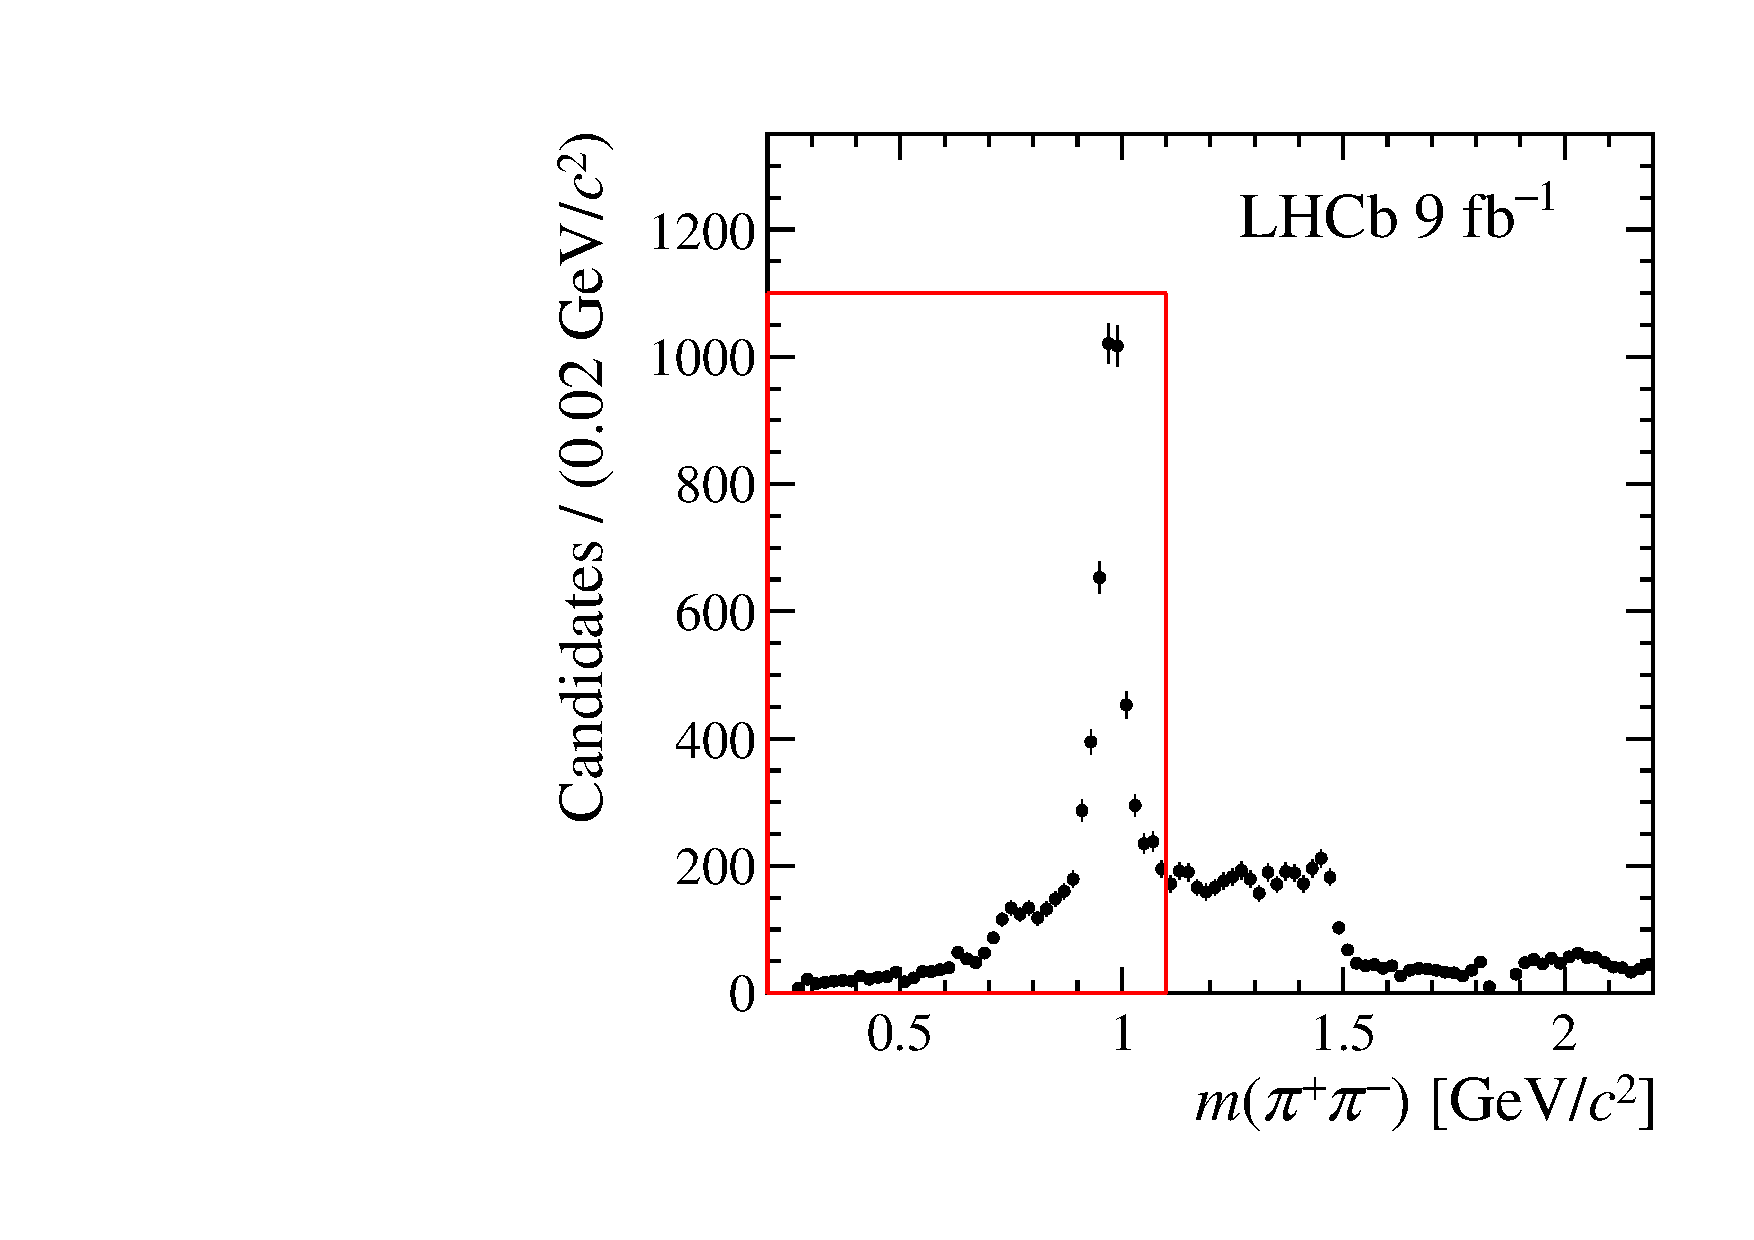
\includegraphics[width=0.4\linewidth]{FigED2b.pdf}
\end{figure}
\end{frame}

\begin{frame}{6. Discussion}
\textbf{Significance and Implications Beyond the SM}\\
\begin{itemize}
    \item Complex phase of the CKM matrix provides CP violation, but is orders of magnitude too small to explain the observed baryon-to-photon ratio $\eta_B \approx 6 \times 10^{-10}$
    \item First observation of CP violation in baryons, offers opportunities to probe for deviations from SM predictions that might reveal new physics
    \item Encourages further experiments to study other baryon decays like $\Ld_{b}^{0}/\Xi_b^0 \to p h^- h^+ h^-$, where $h$ denotes $\pi, K$, dominant diagrams with amplitudes of similar magnitude and significant phase differences
\end{itemize}
\end{frame}

\begin{frame}{1. CP Violation in SM Flavour Physics (Back-up)}
\textbf{What is CP Violation?}\\
\begin{itemize}
    \item Laws of physics are not invariant under the combined operation of charge conjugation (C) and parity (P) transformations
    \item Particles and antiparticles have different behaviours
    \item Required to create matter (Sakharov conditions)
\end{itemize}
\begin{figure}
    \centering
    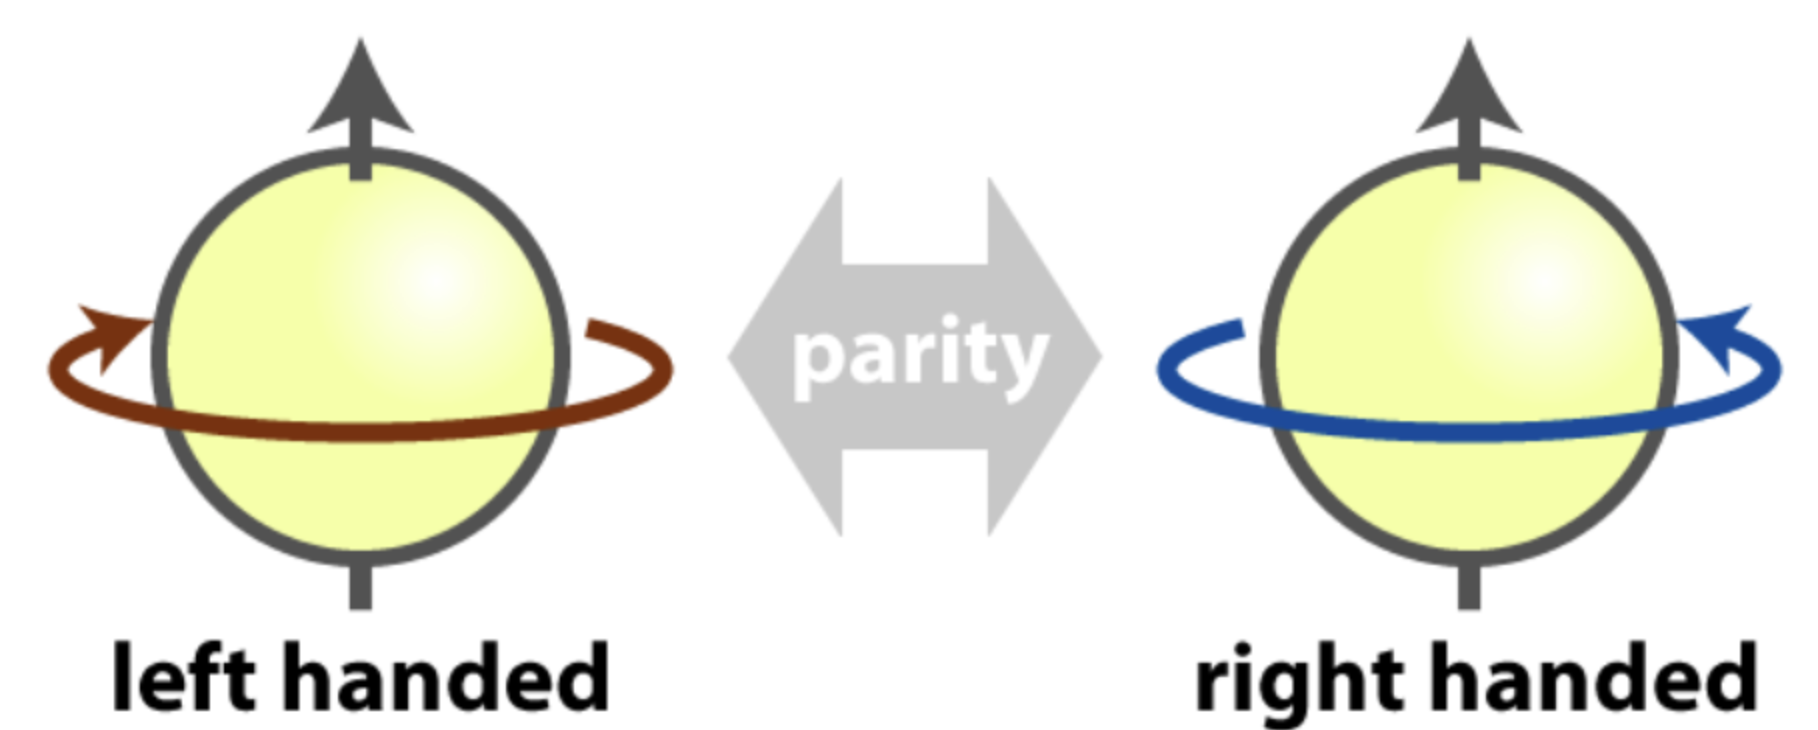
\includegraphics[width=0.5\textwidth]{Parity symmetry.png}
\end{figure}
\br{A. D. Sakharov, 1967}
\end{frame}

\begin{frame}{3. Milestones in CP Violation Detection (Back-up)}
\textbf{Meson Decays Observed}\\
\begin{itemize}
    \item $K_{L}^{0}\to \pi^{+}\pi^{-}$ (1964)
    \item $B^0\to J/\Psi K_{S}^{0}$ (2001)
    \item $D^0 \to K^{+}K^{-}, \pi^{+}\pi^{-}$ (2019)
\end{itemize}
\vspace{10pt}
Despite expectations of similar CP violation in baryons, it had not been observed until this study: $\Ld_{b}^{0}(bud)\to p K^{-}\pi^{-}\pi^{+}$.
\begin{align*}
    \mathcal{A}_{CP}=(2.45\pm0.46\pm0.10)\% \quad (5.2\s)
\end{align*}
\br{J. H. Christenson+, 1964; BaBar, 2001; Belle, 2001; LHCb, 2019}
\end{frame}

\begin{frame}{4. Theoretical Framework for Baryon Decay (Back-up)}
\textbf{Cabibbo–Kobayashi–Maskawa (CKM) Matrix}\\
\begin{itemize}
    \item Only known source of CP symmetry breaking in the Standard Model (SM)
    \begin{align*}
        V_{\mathrm {CKM}}=
        \begin{pmatrix}
            V_{ud} & V_{us} & V_{ub}\\
            V_{cd} & V_{cs} & V_{cb}\\
            V_{td} & V_{ts} & V_{tb}
        \end{pmatrix}, \quad
        \begin{pmatrix}
            d'\\
            s'\\
            b'
        \end{pmatrix}
        =V_{\mathrm{CKM}}
        \begin{pmatrix}
            d\\
            s\\
            b
        \end{pmatrix}
    \end{align*}
    \item Charged-current interaction Lagrangian:
    \begin{align*}
        \La_{\mathrm{C}}=-\frac{g}{\sqrt{2}}\sum_{i, j}\bar{u}_{i}\c^{\mu}P_{L}V_{ij}d_{j}W_{\mu}^{+}+\mathrm{h.c.},
    \end{align*}
    where $g$ is the $SU(2)_{L}$ weak coupling constant, $P_{L}=(1-\c^{5})/2$ is the left-handed projector
\end{itemize}
\end{frame}

\begin{frame}{4. Theoretical Framework for Baryon Decay (Back-up)}
\textbf{Cabibbo–Kobayashi–Maskawa (CKM) Matrix (cont.)}\\
\begin{itemize}
    \item Wolfenstein Parametrization:
    \begin{align*}
        V_{\mathrm{CKM}}=
        \begin{pmatrix}
            1-\frac{\l^2}{2} & \l & A\l^3 (\rho-i\eta)\\
            -\l & 1-\frac{\l^2}{2} & A\l^2\\
            A\l^3 (1-\rho-i\eta) & -A\l^2 & 1
        \end{pmatrix}
        +\bigO(\l^4),
    \end{align*}
    with $\l\approx0.225$, $A\approx0.826$, $\rho\approx0.159$, $\eta\approx0.348$
    \item Highlights hierarchical structure of quark mixing and allows for a convenient approximation accurate up to 0.3\%
\end{itemize}
\end{frame}

\begin{frame}{4. Theoretical Framework for Baryon Decay (Back-up)}
\textbf{Loop-level Process (cont.)}\\
\begin{itemize}
    \item Effective Hamiltonian:
    \begin{align*}
        H_{eff}=\frac{G_{F}}{\sqrt{2}}V_{tb}V_{ts}^\ast\sum_{i}C_{i}\bigO_{i}+\mathrm{h.c.},
    \end{align*}
    where $C_{i}$ are Wilson coefficients that encode loop effects and $\bigO_{i}$ are four-fermion operators, e.g., $(\bar{s}\c^{\mu}b)(\bar{u}\c_{\mu}u)$
    \item $b\to tW^{-}$: vertex $\propto$ $V_{tb}\approx -A\l^2$
    \item $tW^{-}\to s$: vertex $\propto$ $V_{ts}^\ast\approx 1$
    \item Total CKM factor: $\propto$ $V_{tb}V_{us}^\ast$, weak phase $\phi_{L}=\arg(V_{tb}V_{us}^\ast)\approx 0$
\end{itemize}
\begin{figure}
    \centering
    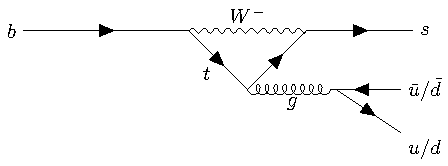
\includegraphics[width=0.6\linewidth]{b_loop.pdf}
\end{figure}
\end{frame}

\end{document}